\chapter[Installation]{Installation}

\section{Configuration}

Une configuration minimale est requise pour l'utilisation de ce logiciel. En effet, le programme étant codé en Python 3, il est nécessaire que cette version soit prise en compte sur l'ordinateur. \\

Des packages particuliers de Python doivent également être installés avant le lancement du programme :

\renewcommand{\arraystretch}{1.7}
\begin{figure}[H]
	\begin{center}
		\begin{tabular}{|c|m{.7\textwidth}|}
			\hline
			Package Python & Installation sous Ubuntu \\
			\hline
			PyQt5 & 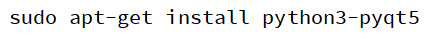
\includegraphics[scale=0.65]{install_pyqt5.png}  \\
			PyShp & 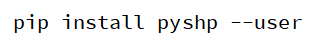
\includegraphics[scale=0.65]{install_pyshp.png} \\
			gdal & 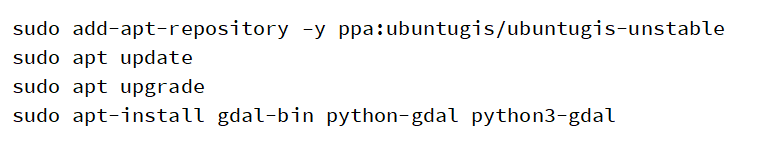
\includegraphics[scale=0.65]{install_gdal.png} \\
			qimage2ndarray & 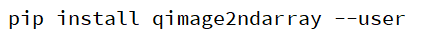
\includegraphics[scale=0.65]{install_qimage2ndarray.png} \\
			\hline
		\end{tabular}
	\end{center}
	\caption[Installation minimale sous Ubuntu]{Installation minimale sous Ubuntu}
	\label{tab:installubuntu}
\end{figure}

\renewcommand{\arraystretch}{1.7}
\begin{figure}[H]
	\begin{center}
		\begin{tabular}{|c|m{.7\textwidth}|}
			\hline
			Package Python & Installation sous Windows \\
			\hline
			PyQt5 & Documentation en ligne de PyQt5 : \newline
							\textit{http://pyqt.sourceforge.net/Docs/PyQt5/installation.html} \\
			PyShp & Installation du package dans Anaconda : \newline
							\textit{https://anaconda.org/pelson/pyshp} \\
			gdal & Documentation en ligne de gdal :\newline
							\textit{https://gdal.gloobe.org/install.html} \\
			qimage2ndarray & Documentation en ligne :\newline
							\textit{https://pypi.python.org/pypi/qimage2ndarray}\\
			\hline
		\end{tabular}
	\end{center}
	\caption[Installation minimale sous Windows]{Installation minimale sous Windows}
	\label{tab:installwindowsu}
\end{figure}

\section{Fichiers nécessaires}

\noindent Pour le bon fonctionnement du programme, il est nécessaire d'avoir dans un dossier unique :
\begin{itemize}[label=$\rightarrow$]
	\item le fichier \textit{interface.py}
	\item les fichiers \textit{classificationActive.py}, \textit{chargementFichiers.py}, \textit{choixClasse.py}
	\item les fichiers \textit{building.py}, \textit{background.py}, \textit{strategy.py}
\end{itemize}

\section{Données du programme}

\noindent Les données en entrée du programme doivent respecter un formalisme minimal :
\begin{itemize}[label=$\rightarrow$]
	\item le fichier de définition des classes doit être au format .CSV, et comporter deux colonnes sans en-tête (nom et description de la classe).
	\item le fichier des résultats de l'auto-qualification doit être au format .CSV, et comporter trois colonnes sans en-tête (identifiant, classe et probabilité).
	\item le dossier des emprises doit contenir un fichier .SHP par entité. Ces emprises doivent être dans le même système de coordonnées que l'orthoimage.
	\item l'orthoimage couleur doit être au format .GEOTIFF. Elle doit être superposables aux emprises.
\end{itemize}
